% LHCb Template by Dylan J. White
% Precursor by Rupert Tombs
\documentclass[a4paper]{article}

% packages
\usepackage{amsmath}
\usepackage{graphicx}
\usepackage{hyperref}
\usepackage[margin=2.75 cm]{geometry} % margins
\usepackage{tikz}
\usepackage[compat=1.1.0]{tikz-feynman}
\usepackage[font=small,labelfont=bf]{caption}
\usepackage{subcaption}
\usepackage{amsmath} % adds a large collection of math symbols
\usepackage{amssymb}
\usepackage{amsfonts}
\usepackage{upgreek} % adds support for greek letters in roman typeset
\usepackage{multirow}
\usepackage{ifthen} 
\newboolean{uprightparticles}
\setboolean{uprightparticles}{false} %Set true for upright
%\usepackage[section]{placeins}

% inputs
\input{lhcb-symbols-def} % add in the predefined LHCb symbols

\begin{document}

% cover
\begin{center}
\Huge{\bf Report title goes here} \vskip 40pt
\normalsize{\emph{Author Name}}\vskip 20pt
School of Physics and Astronomy\vskip 2pt
The University of Manchester\vskip 20pt
Report\vskip 20pt
September 2018\vskip 20pt

%This project was performed in collaboration with
%\normalsize{\emph{Partner name}}
\end{center}\vskip 96pt





% *** ABSTRACT ***
\section*{Abstract}
\label{sec:abstract}
A brief description of the enclosed work.
\vskip 64pt


\tableofcontents


\clearpage % break page





% *** INTRODUCTION ***
\section{Introduction}
\label{sec:introduction}
This is a template for reports that use \lhcb symbols, such as \DFourpi.





% *** DETECTOR ***
\section{Detector}
\label{sec:detector}
This section can usually be taken verbatim from \lhcb collaboration writing guidelines.





% *** THEORY ***
\section{Theory}
\label{sec:theory}



\subsection{Figures}
\label{sec:theory_figures}
Figures can be included as shown.

\begin{figure}[ht]
    \centering
    % trim=left bottom right top
    \includegraphics[clip, trim=0.5cm 2cm 0.5cm 0cm,width=0.7\textwidth]{figures/lhcb.pdf}
    \caption{Diagram of the \lhcb detector \cite{LHCbDetectorGeometry}.}
    \label{fig:lhcb}
\end{figure}

\subsubsection{Subfigures}
\label{sec:theory_figures_subfigures}
To have images side-by-side with separate labels, use subfigures.

\begin{figure}[ht]
    \centering
    \begin{subfigure}{0.49\textwidth}
        \centering
        \includegraphics[clip, trim=0.5cm 2cm 0.5cm 0cm,width=1\textwidth]{figures/lhcb.pdf}
        \subcaption{\lhcb}
    \end{subfigure}
    \begin{subfigure}{0.49\textwidth}
        \centering
        \includegraphics[clip, trim=0.5cm 2cm 0.5cm 0cm,width=1\textwidth]{figures/lhcb.pdf}
        \subcaption{\lhcb}
    \end{subfigure}
    \caption{Two diagrams of the \lhcb detector \cite{LHCbDetectorGeometry}.}
    \label{fig:pvalsFiducial2k2piPodd}
\end{figure}



\subsection{Equations}
\label{sec:theory_equations}
Provided example equations include

\begin{equation}
    C_{T}=\vec{p}_{a} \cdot (\vec{p}_{b} \times \vec{p}_{c}),
    \label{eq:triple_product}
\end{equation}

\begin{equation}
    T=\sum^{n}_{i,j>i}\frac{\psi_{ij}}{n(n-1)}+\sum^{\overline{n}}_{i,j>i}\frac{\psi_{ij}}{\overline{n}(\overline{n}-1)}-\sum^{n,\overline{n}}_{i,j}\frac{\psi_{ij}}{n\overline{n}},
    \label{eq:et_test_statistic}
\end{equation}

\begin{equation}
    \begin{bmatrix}
        d' \\
        s' \\
        b'
    \end{bmatrix}
    =
    \begin{bmatrix}
        \Vud & \Vus & \Vub \\
        \Vcd & \Vcs & \Vcb \\
        \Vtd & \Vts & \Vtb
    \end{bmatrix}
    \begin{bmatrix}
        d \\
        s \\
        b
    \end{bmatrix},
    \label{eq:CKM_general}
\end{equation}

\noindent where the \texttt{\textbackslash noindent} command is used for formatting when an equation is part of a sentence.

\subsubsection{Subequations}
\label{sec:theory_equations_subequations}
Similarly to figures, equations can be grouped using subequations.

\begin{subequations}
\begin{equation}
    M=|M|e^{i\theta}e^{i\phi},
\end{equation}
\begin{equation}
    \overline{M}=|M|e^{i\theta}e^{-i\phi}.
\end{equation}
\end{subequations}



\subsection{Tables}
\label{sec:theory_tables}
Tables are used to display information in bulk.

\begin{table}[h]
    \centering
    \begin{tabular}{c c||c c|c c}
        & & \multicolumn{2}{c}{Fiducial up} & \multicolumn{2}{c}{Fiducial down}\\
        & & $\chi^{2}$ & KS & $\chi^{2}$ & KS \\\hline
        \multirow{2}{*}{$\pi\pi\pi\pi$} & \PP-even & 0.56 & 0.98 & 0.39 & 0.56 \\
        & \PP-odd & 0.98 & 1.00 & 0.79 & 0.33 \\\hline
        \multirow{2}{*}{$KK\pi\pi$} & \PP-even & 0.67 & 0.98 & 0.90 & 0.98 \\
        & \PP-odd & 0.83 & 0.56 & 0.78 & 1.00
    \end{tabular}
    \caption{Selection of numbers, arranged in a sensible way for ease of comprehension.}
    \label{tab:pvalsFiducial}
\end{table}

Rows are separated using a double backslash, \textbackslash\textbackslash. Cells are separated by ampersands, \&. Vertical lines, as well as horizontal text alignment, is determined in the bracket following \texttt{\textbackslash begin\{tabular\}}. Horizontal lines are added using the \texttt{\textbackslash hline} command. The \texttt{\textbackslash multirow} and \texttt{\textbackslash multicolumn} commands are used for cells that span multiple rows and columns respectively.



% start a new page
\clearpage

\subsection{Feynman diagrams}
\label{sec:theory_feynman}
Feynman diagrams can be created using the TikZ-Feynman package. For these to work, you must compile using the LuaLaTeX compiler.

\begin{figure}[ht]
    \centering
    \feynmandiagram[horizontal=a to b]{
        i1 [particle=\(e^{-}\)] -- [fermion] a -- [fermion] i2 [particle=\(e^{+}\)],
        a -- [photon, edge label=\(\gamma\), momentum'=\(k\)] b,
        f1 [particle=\(\mu^{+}\)] -- [fermion] b -- [fermion] f2 [particle=\(\mu^{-}\)],
    };
    \caption{Example Feynman diagram using auto-positioning.}
    \label{fig:feynman_1}
\end{figure}

\begin{figure}[ht]
    \centering
    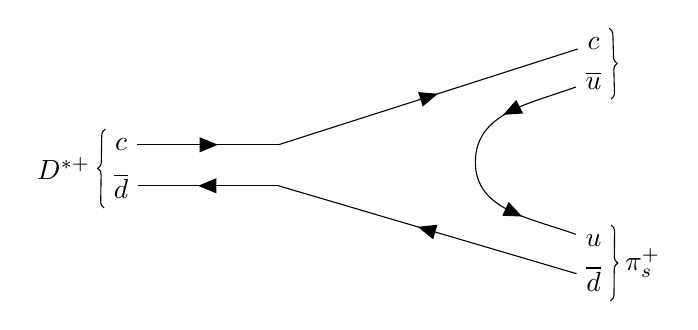
\begin{tikzpicture}
    \begin{feynman}
        \vertex (root);
        % initial
        \vertex [above=0.02cm of root] (1_c) {\(c\)};
        \vertex [below=0.02cm of root] (1_db) {\(\overline{d}\)};
        % middle
        \vertex [right=2cm of 1_c] (a_q1);
        \vertex [right=2cm of 1_db] (a_q2);
        \vertex [right=4.5cm of root] (b_q);
        % final
        \vertex [right=6cm of root] (2_mid);
        \vertex [above=1.3cm of 2_mid] (2_c) {\(c\)};
        \vertex [above=0.8cm of 2_mid] (2_ub) {\(\overline{u}\)};
        \vertex [below=0.8cm of 2_mid] (2_u) {\(u\)};
        \vertex [below=1.2cm of 2_mid] (2_db) {\(\overline{d}\)};
        
        \diagram* {
            (1_c) -- [fermion] (a_q1) -- [fermion] (2_c),
            (2_db) -- [fermion] (a_q2) -- [fermion] (1_db),
            (2_ub) -- [fermion, out=-160, in=90] (b_q) -- [fermion, out=-90, in=160] (2_u),
        };
        
        \draw [decoration={brace}, decorate] (1_db.south west) -- (1_c.north west)
          node [pos=0.5, left] {\(D^{\ast+}\,\)};
        \draw [decoration={brace}, decorate]  (2_c.north east) -- (2_ub.south east)
          node [pos=0.5, right] {\(\,\Dz\)};
        \draw [decoration={brace}, decorate] (2_u.north east) -- (2_db.south east)
          node [pos=0.5, right] {\(\,\pi^{+}_{s}\)};
    \end{feynman}
    \end{tikzpicture}
    \caption{Example Feynman diagram using custom vertex positioning.}
    \label{fig:quarkFlowDstar}
\end{figure}

\subsubsection{Subfigures with Feynman Diagrams}

\begin{figure}[ht]
    \centering
    \begin{subfigure}[t]{0.35\textwidth}
        \centering
        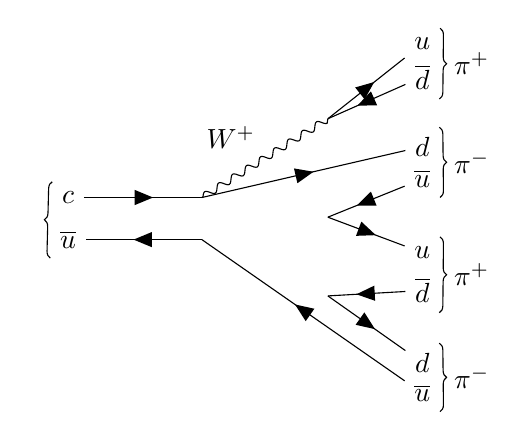
\begin{tikzpicture}
        \begin{feynman}
            \vertex (root);
            % initial
            \vertex [above=0.05cm of root] (1_c) {\(c\)};
            \vertex [below=0.05cm of root] (1_ub) {\(\overline{u}\)};
            % middle
            \vertex [right=1.7cm of 1_c] (a_q1);
            \vertex [right=1.7cm of 1_ub] (a_q2);
            \vertex [right=3.3cm of root] (b_root);
            \vertex [above=1.25cm of b_root] (b_W);
            \vertex [above=0cm of b_root] (b_23);
            \vertex [below=1cm of b_root] (b_34);
            % final
            \vertex [right=4.5cm of root] (2_mid);
            \vertex [above=2cm of 2_mid] (2_1_u) {\(u\)};
            \vertex [above=1.5cm of 2_mid] (2_1_db) {\(\overline{d}\)};
            \vertex [above=0.65cm of 2_mid] (2_2_d) {\(d\)};
            \vertex [above=0.25cm of 2_mid] (2_2_ub) {\(\overline{u}\)};
            \vertex [below=0.25cm of 2_mid] (2_3_u) {\(u\)};
            \vertex [below=0.65cm of 2_mid] (2_3_db) {\(\overline{d}\)};
            \vertex [below=1.6cm of 2_mid] (2_4_d) {\(d\)};
            \vertex [below=2cm of 2_mid] (2_4_ub) {\(\overline{u}\)};
            
            \diagram* {
                (1_c) -- [fermion] (a_q1) -- [fermion] (2_2_d),
                (2_4_ub) -- [fermion] (a_q2) -- [fermion] (1_ub),
                (a_q1) -- [boson, edge label=\(W^{+}\)] (b_W),
                (2_1_db) -- [fermion] (b_W) -- [fermion] (2_1_u),
                (2_2_ub) -- [fermion] (b_23) -- [fermion] (2_3_u), %, out=-160, in=45] (b_root) -- [fermion,     out=-45, in=160
                (2_3_db) -- [fermion] (b_34) -- [fermion] (2_4_d), %, out=-160, in=45] (b_root) -- [fermion,     out=-45, in=160
            };
            
            \draw [decoration={brace}, decorate] (1_ub.south west) -- (1_c.north west)
                node [pos=0.5, left] {\(\Dz\,\)};
            \draw [decoration={brace}, decorate]  (2_1_u.north east) -- (2_1_db.south east)
                node [pos=0.5, right] {\(\,\pi^{+}\)};
            \draw [decoration={brace}, decorate] (2_2_d.north east) -- (2_2_ub.south east)
                node [pos=0.5, right] {\(\,\pi^{-}\)};
            \draw [decoration={brace}, decorate]  (2_3_u.north east) -- (2_3_db.south east)
                node [pos=0.5, right] {\(\,\pi^{+}\)};
            \draw [decoration={brace}, decorate] (2_4_d.north east) -- (2_4_ub.south east)
                node [pos=0.5, right] {\(\,\pi^{-}\)};
        \end{feynman}
        \end{tikzpicture}
        \caption{Tree-level diagram}
    \end{subfigure}
    ~~~~~~~~~~~~~~
    \begin{subfigure}[t]{0.35\textwidth}
        \centering
        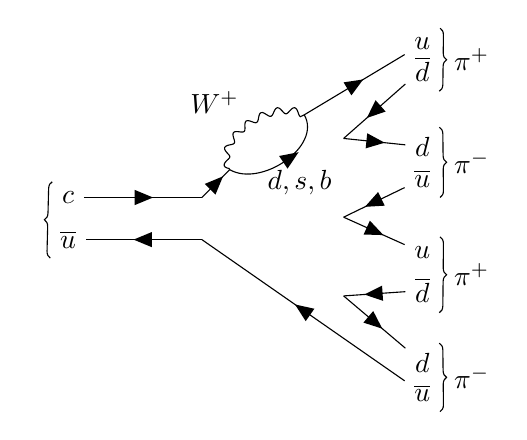
\begin{tikzpicture}
        \begin{feynman}
            \vertex (root);
            % initial
            \vertex [above=0.05cm of root] (1_c) {\(c\)};
            \vertex [below=0.05cm of root] (1_ub) {\(\overline{u}\)};
            % middle
            \vertex [right=1.7cm of 1_c] (a_q1);
            \vertex [right=1.7cm of 1_ub] (a_q2);
            \vertex [above right=0.5cm of a_q1] (a_W);
            \vertex [right=3.5cm of root] (b_root);
            \vertex [above=1.3cm of b_root] (b_W_temp);
            \vertex [left=0.5cm of b_W_temp] (b_W);
            \vertex [above=1cm of b_root] (b_12);
            \vertex [above=0cm of b_root] (b_23);
            \vertex [below=1cm of b_root] (b_34);
            % final
            \vertex [right=4.5cm of root] (2_mid);
            \vertex [above=2cm of 2_mid] (2_1_u) {\(u\)};
            \vertex [above=1.6cm of 2_mid] (2_1_db) {\(\overline{d}\)};
            \vertex [above=0.65cm of 2_mid] (2_2_d) {\(d\)};
            \vertex [above=0.25cm of 2_mid] (2_2_ub) {\(\overline{u}\)};
            \vertex [below=0.25cm of 2_mid] (2_3_u) {\(u\)};
            \vertex [below=0.65cm of 2_mid] (2_3_db) {\(\overline{d}\)};
            \vertex [below=1.6cm of 2_mid] (2_4_d) {\(d\)};
            \vertex [below=2cm of 2_mid] (2_4_ub) {\(\overline{u}\)};
            
            \diagram* {
                (1_c) -- [fermion] (a_q1) -- [fermion] (a_W),
                (2_4_ub) -- [fermion] (a_q2) -- [fermion] (1_ub),
                (a_W) -- [boson, out=120, in=150, edge label=\(W^{+}\)] (b_W) -- [anti fermion, out=-60, in=-30, edge label={\(\!\!\!\!\!\!d,s,b\)}] (a_W), % 
                (b_W) -- [fermion] (2_1_u),
                (2_1_db) -- [fermion] (b_12) -- [fermion] (2_2_d), %, out=-160, in=45] (b_root) -- [fermion,     out=-45, in=160
                (2_2_ub) -- [fermion] (b_23) -- [fermion] (2_3_u), %, out=-160, in=45] (b_root) -- [fermion,     out=-45, in=160
                (2_3_db) -- [fermion] (b_34) -- [fermion] (2_4_d), %, out=-160, in=45] (b_root) -- [fermion,     out=-45, in=160
            };
            
            \draw [decoration={brace}, decorate] (1_ub.south west) -- (1_c.north west)
                node [pos=0.5, left] {\(\Dz\,\)};
            \draw [decoration={brace}, decorate]  (2_1_u.north east) -- (2_1_db.south east)
                node [pos=0.5, right] {\(\,\pi^{+}\)};
            \draw [decoration={brace}, decorate] (2_2_d.north east) -- (2_2_ub.south east)
                node [pos=0.5, right] {\(\,\pi^{-}\)};
            \draw [decoration={brace}, decorate]  (2_3_u.north east) -- (2_3_db.south east)
                node [pos=0.5, right] {\(\,\pi^{+}\)};
            \draw [decoration={brace}, decorate] (2_4_d.north east) -- (2_4_ub.south east)
                node [pos=0.5, right] {\(\,\pi^{-}\)};
        \end{feynman}
        \end{tikzpicture}
        \caption{Penguin diagram}
    \end{subfigure}
    ~~~~
    \caption{Two \DFourpi decay modes shown together by using Feynman diagrams with subfigures.}
    \label{fig:quarkFlowFourPi}
\end{figure}




% ***** MORE SECTIONS *****
\section{More sections go here}

% ***** CONCLUSION *****
\section{Conclusion}
A summary of the results, and some suggestions for future work.





\bibliography{bib}{}
\bibliographystyle{unsrt}

\end{document}